\chapter{\texorpdfstring{Occurrence Graph}{Occurrence Graph}}
\label{ch:09}
\lecturemeta{Lezione 09 \quad\textbullet\quad 2026-07-03 \quad\textbullet\quad Roberto Bruni}{Petri nets · Esparza, \emph{Free Choice Petri Nets} (optional)}

In \hyperref[ch:08]{08 — Nets Intro} abbiamo definito l'insieme delle marcature raggiungibili $[M_0\rangle$ di un Petri net: tutti gli stati in cui il processo può finire. Ma un \emph{insieme} di stati non basta per ragionare sul comportamento — vogliamo sapere anche \emph{come} si passa da uno stato all'altro. Questa lezione organizza quegli stati in un \textbf{grafo}, l'\textbf{occurrence graph}, e lo usa per rispondere a una domanda fondamentale: il processo può accumulare token all'infinito, o resta "limitato"? È la nozione di \textbf{boundedness}, e quando il grafo diventa infinito introdurremo un'approssimazione finita, il \textbf{coverability graph}.

\section{\texorpdfstring{L'occurrence graph (reachability graph)}{L'occurrence graph (reachability graph)}}

L'idea è semplice: prendiamo tutte le marcature raggiungibili come \textbf{nodi} e colleghiamole con archi ogni volta che uno scatto porta dall'una all'altra.

\begin{boxdefinition}{Occurrence graph (aka Reachability graph)}
L'\textbf{occurrence graph} di una rete $N$ con marcatura iniziale $M_0$ è il grafo $OG(N) = ([M_0\rangle, A)$ dove: - i \textbf{nodi} sono le \textbf{marcature raggiungibili} $[M_0\rangle$; - gli \textbf{archi} sono gli \textbf{scatti}: $A \subseteq [M_0\rangle \times T \times [M_0\rangle$ con $(M, t, M') \in A$ se e solo se $M \xrightarrow{t} M'$.

In pratica: un nodo per ogni stato raggiungibile, un arco etichettato $t$ per ogni scatto possibile tra due stati.
\end{boxdefinition}

Rappresenta \textbf{tutte le possibili occurrence sequence} della rete in un colpo solo: ogni cammino nel grafo, a partire da $M_0$, è una sequenza di scatti eseguibile.

\subsection{\texorpdfstring{Come si calcola}{Come si calcola}}

L'algoritmo è una classica esplorazione a \textbf{worklist} (lista di lavoro): si tiene un insieme \texttt{Todo} di marcature ancora da esplorare, e si espande finché non è vuoto.

\begin{boxdefinition}{Algoritmo per $OG(N)$}
\begin{enumerate}
\item Inizializza \texttt{Nodes = \{\}}, \texttt{Arcs = \{\}}, \texttt{Todo = \{M0\}}.
\item Estrai una marcatura $M$ da \texttt{Todo}.
\item Aggiungila ai \texttt{Nodes} (e toglila da \texttt{Todo}).
\item Calcola tutti gli scatti da $M$: \texttt{Firings = \{(M, t, M') | M —t→ M'\}}.
\item Individua le marcature \textbf{nuove} (\texttt{New}), cioè quelle in \texttt{Firings} non ancora in \texttt{Nodes} né in \texttt{Todo}.
\item Aggiungi \texttt{New} a \texttt{Todo} e \texttt{Firings} agli \texttt{Arcs}.
\item Se \texttt{Todo} è vuoto, \textbf{stop}; altrimenti torna al passo 2.
\end{enumerate}
\end{boxdefinition}

\subsection{\texorpdfstring{Un esempio: il semaforo}{Un esempio: il semaforo}}

Consideriamo un semaforo modellato come una rete: un solo token che circola tra i place \texttt{red}, \texttt{green}, \texttt{yellow}, con le transizioni \texttt{go-green}, \texttt{go-yellow}, \texttt{go-red}. Poiché c'è \textbf{un solo token} e cicla, l'occurrence graph è un semplice ciclo di tre stati.

\begin{figure}[!htb]
\centering
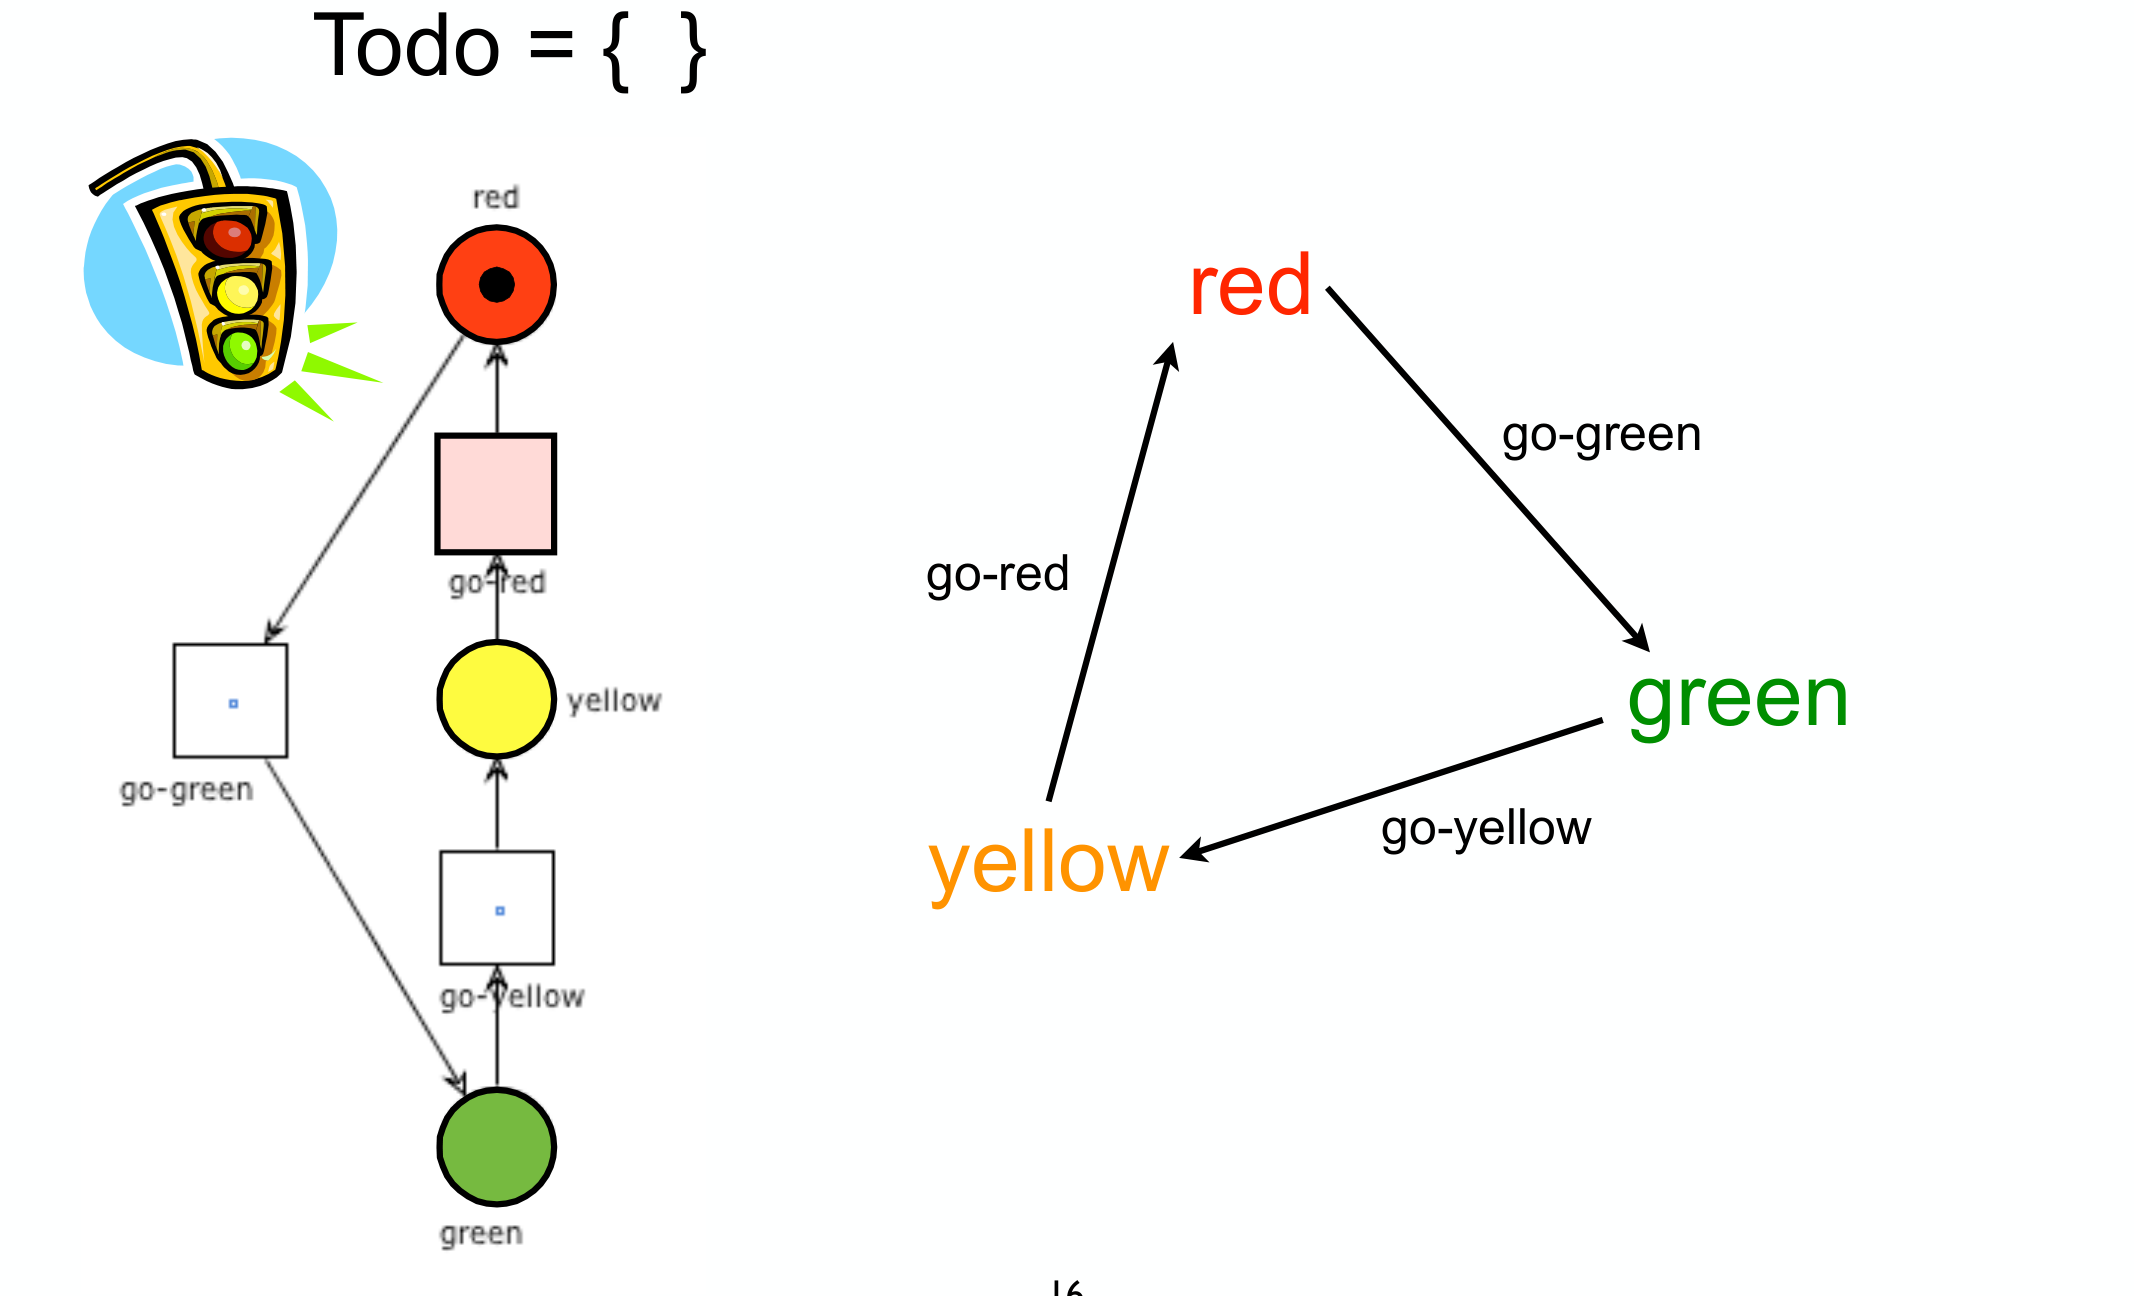
\includegraphics[width=0.74\linewidth,height=0.34\textheight,keepaspectratio]{images/09-occurrence_p9_traffic-light.png}
\caption{Semaforo singolo. La rete (sinistra) ha un solo token; il suo occurrence graph (destra) è il ciclo \texttt{red → green → yellow → red}. Ogni stato è una marcatura con il token in un place.}
\end{figure}

\subsection{\texorpdfstring{Il product state space: due semafori}{Il product state space: due semafori}}

La situazione diventa interessante — e mostra la vera natura dei Petri net — con \textbf{due semafori indipendenti} che funzionano in parallelo. Ora lo stato è una coppia (un token in ciascun semaforo), e le marcature raggiungibili sono tutte le \textbf{combinazioni} dei tre stati di un semaforo con i tre dell'altro: $3 \times 3 = 9$ nodi.

\begin{figure}[!htb]
\centering
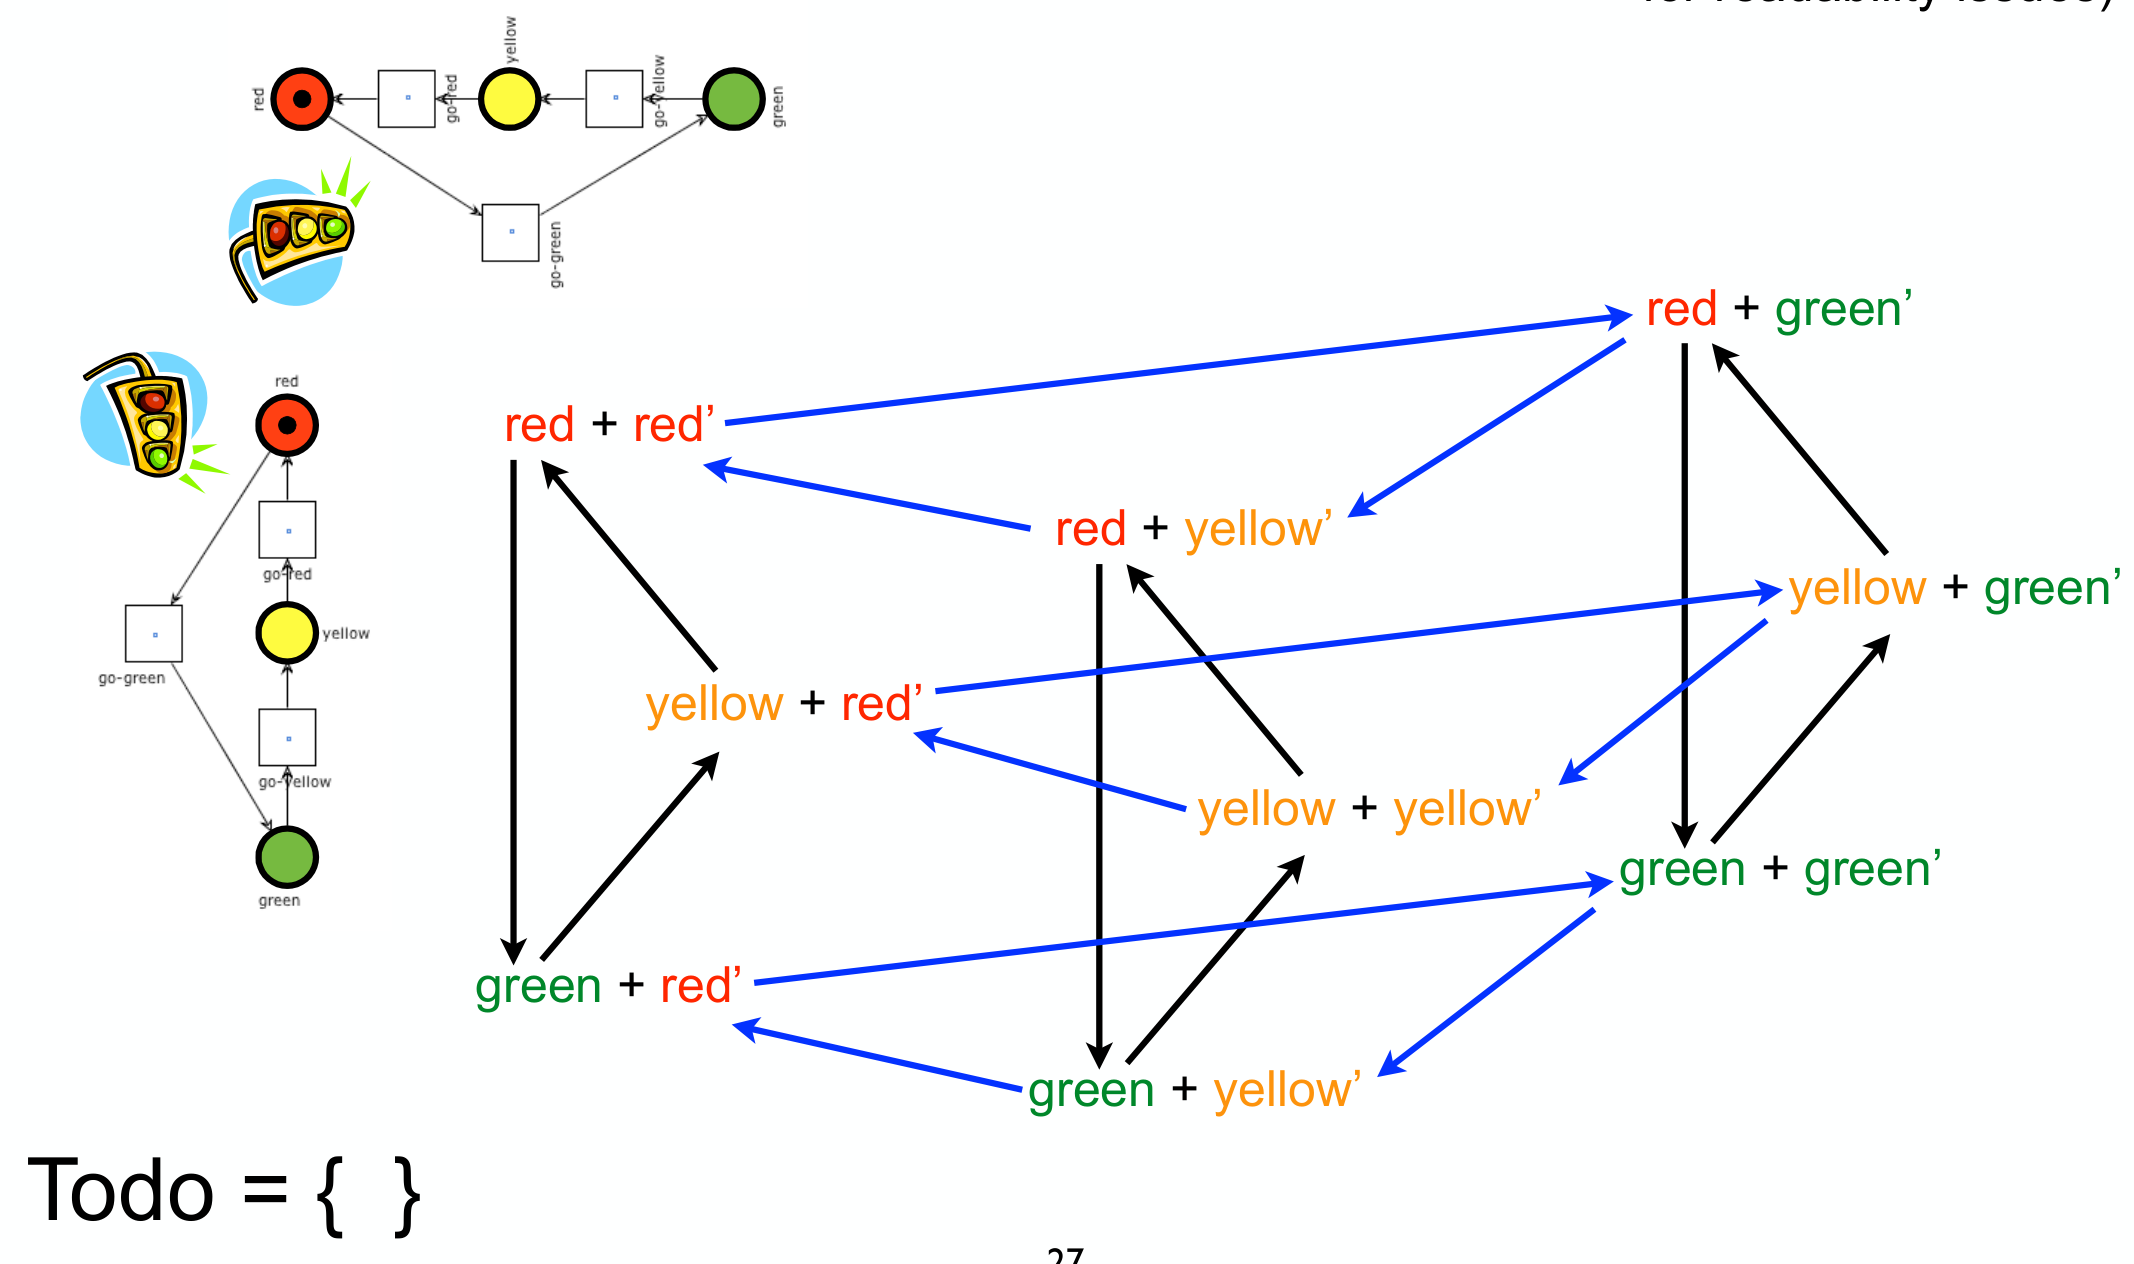
\includegraphics[width=0.74\linewidth,height=0.34\textheight,keepaspectratio]{images/09-occurrence_p20_two-lights-rg.png}
\caption{Due semafori. L'occurrence graph ha \textbf{9 stati}, ognuno una marcatura \texttt{x + y'} con $x$ stato del primo semaforo e $y'$ del secondo. Da ogni nodo partono due archi (uno per semaforo che avanza): è la \textbf{concorrenza} resa esplicita come intreccio di scatti indipendenti. Nota come il numero di stati \textbf{cresce moltiplicativamente} col numero di componenti.}
\end{figure}

Questo esempio illustra sia il pregio (i Petri net rappresentano la concorrenza in modo compatto: la \emph{rete} dei due semafori è piccola) sia il costo (l'\emph{occurrence graph} esplode: due componenti da 3 stati danno 9 nodi, dieci componenti darebbero $3^{10}$).

\section{\texorpdfstring{Boundedness: il processo può "traboccare"?}{Boundedness: il processo può "traboccare"?}}

Una domanda cruciale per l'analisi: esiste un limite al numero di token che un place può contenere? Se sì, quel place non può "overflow"; se no, il sistema può accumulare risorse senza fine (spesso un bug).

\begin{boxdefinition}{k-boundedness, safe, bounded}
\begin{itemize}
\item Un place $p$ è \textbf{k-bounded} se \textbf{nessuna} marcatura raggiungibile ha più di $k$ token in $p$.
\item Una rete è \textbf{k-bounded} se tutti i suoi place lo sono ($k$ è allora un limite di capacità imponibile senza rischio di overflow).
\item Un place è \textbf{safe} se è \textbf{1-bounded} (al più un token); una rete è safe se tutti i suoi place lo sono.
\item Un place è \textbf{bounded} se è k-bounded \textbf{per qualche} $k$; una rete è \textbf{bounded} se tutti i place lo sono, \textbf{unbounded} altrimenti (esiste un place in cui può comparire un numero arbitrario di token).
\end{itemize}
\end{boxdefinition}

Formalmente, una rete è bounded se:

\[
\exists k \in \mathbb{N}.\; \forall M \in [M_0\rangle.\; \forall p \in P.\; M(p) \le k
\]

\subsection{\texorpdfstring{Il legame con l'occurrence graph}{Il legame con l'occurrence graph}}

C'è un teorema semplice ma potentissimo che collega una proprietà del \emph{comportamento} (boundedness) a una proprietà del \emph{grafo} (finitezza).

\begin{boxtheorem}{Boundedness $\Longleftrightarrow$ finitezza del reachability graph}
Una rete è \textbf{bounded} se e solo se il suo occurrence graph è \textbf{finito}.

\emph{($\Rightarrow$) Bounded implica finito.} Se è k-bounded, ogni place ha al più $k$ token; con $n$ place ci sono al più $(k+1)^n$ marcature possibili, quindi un numero finito di nodi.

\emph{($\Leftarrow$) Finito implica bounded.} Se il grafo è finito, per ogni nodo $M$ prendiamo $k_M$ = massimo numero di token in uno stesso place.

\[
k = \max\{k_M\}
\]

Questo massimo esiste perché i nodi sono finiti. Allora la rete è k-bounded. $\blacksquare$
\end{boxtheorem}

Come conseguenza immediata: \textbf{una rete è unbounded se e solo se il suo reachability graph è infinito}. Questo ci dà un metodo per rilevare l'unboundedness — ma anche un problema: se il grafo è infinito, l'algoritmo di prima \textbf{non termina}. Serve un'approssimazione finita.

\section{\texorpdfstring{Coverability graph: domare l'infinito}{Coverability graph: domare l'infinito}}

Quando la rete è unbounded, il reachability graph ha infiniti nodi e non lo possiamo costruire. Il \textbf{coverability graph} è una sua \textbf{sovra-approssimazione finita}: ammette marcature "con infiniti token" in un place, rappresentati dal simbolo $\omega$ (o $\infty$).

\begin{boxdefinition}{Coverability graph}
Una sovra-approssimazione \textbf{finita} del reachability graph, che ammette marcature con \textbf{infiniti token} in un place. I nodi non sono più marcature ordinarie ma \textbf{extended bag} $B : P \to \mathbb{N} \cup \{\omega\}$, dove $\omega$ marca un place \textbf{illimitato}.
\end{boxdefinition}

L'idea per scoprire i place illimitati sfrutta la \textbf{monotonicità} dei Petri net (se una sequenza è abilitata in una marcatura, lo è anche in una marcatura più grande):

\begin{boxtip}{Come si scopre un place unbounded}
Supponiamo che lungo il calcolo si trovi $M_0 \xrightarrow{\;\ast\;} M \xrightarrow{\;\ast\;} M'$ con $M \subset M'$ (la seconda marcatura contiene \textbf{strettamente} la prima). Sia $L = M' - M$ il "surplus" di token prodotto. Per monotonicità possiamo ripetere la stessa sequenza all'infinito: \(M \xrightarrow{\;\ast\;} M+L \xrightarrow{\;\ast\;} M+2L \xrightarrow{\;\ast\;} \cdots \xrightarrow{\;\ast\;} M+nL\) Quindi \textbf{ogni place $p$ con $L(p) > 0$ è unbounded}: nell'extended bag lo segniamo con $\omega$ al posto del suo valore.
\end{boxtip}

Le operazioni sugli extended bag estendono quelle sui multiset trattando $\omega$ come "assorbente":

\[
\begin{aligned}
\omega + n &= \omega \\
\omega - n &= \omega \\
\omega &\ge n \quad \text{per ogni } n \text{ finito}
\end{aligned}
\]

L'algoritmo del coverability graph è come quello del reachability graph, ma quando crea una nuova marcatura $B'$ controlla se lungo il cammino esiste un antenato $B'' \subset B'$: per ogni place dove $B''(p) < B'(p)$, mette $\omega$.

\begin{figure}[!htb]
\centering
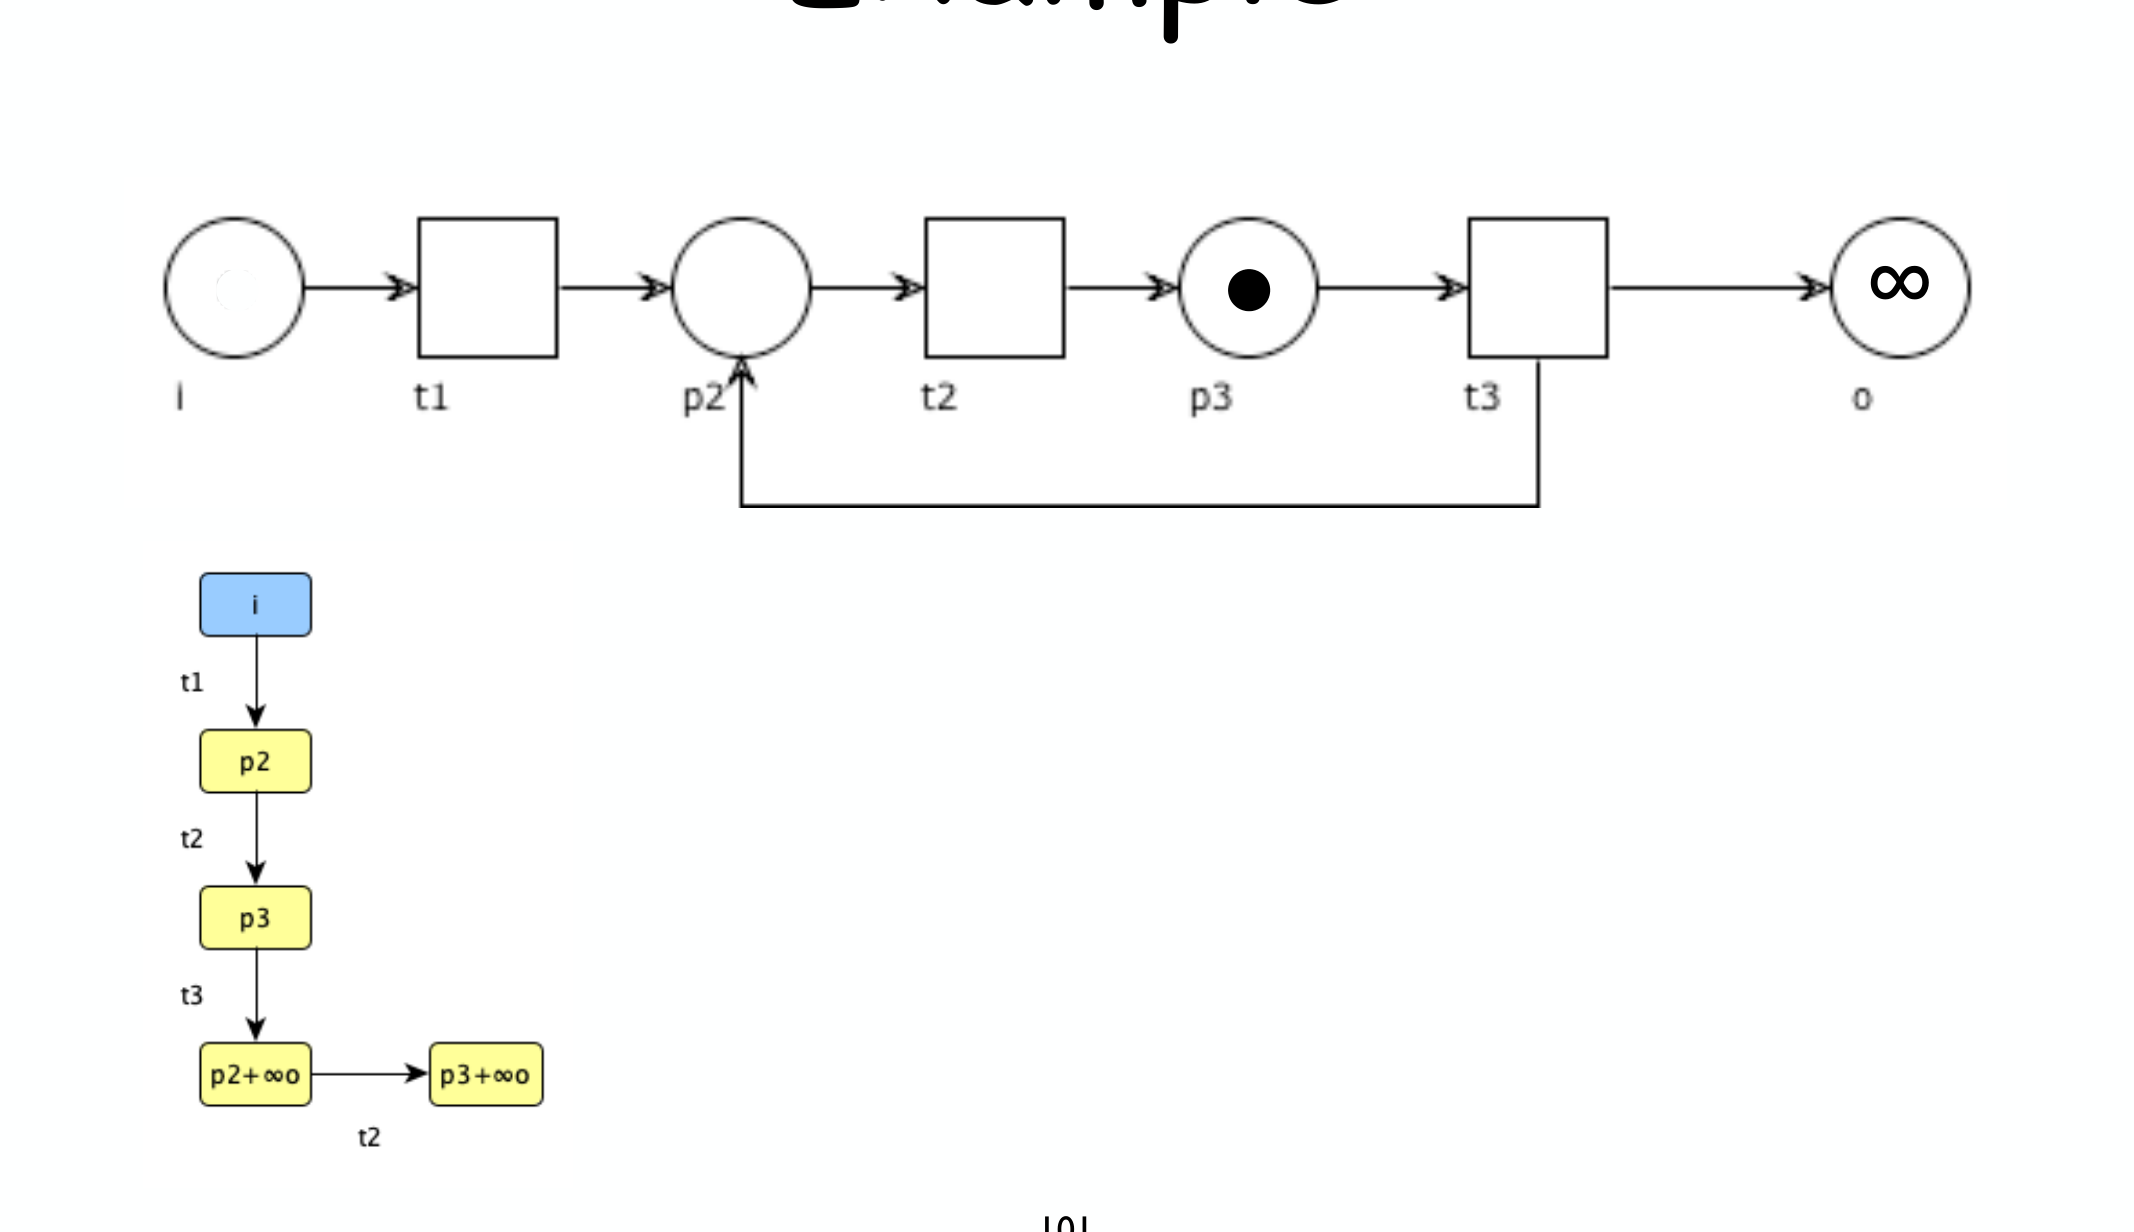
\includegraphics[width=0.74\linewidth,height=0.34\textheight,keepaspectratio]{images/09-occurrence_p89_coverability.png}
\caption{Coverability graph. La rete ha un ciclo che a ogni giro deposita un token in \texttt{o} senza mai consumarlo: \texttt{o} è \textbf{unbounded}, marcato $\infty$. Il grafo resta \textbf{finito} grazie a $\omega$: invece di enumerare \texttt{o, 2o, 3o, ...} (infiniti nodi) si collassa tutto in \texttt{∞o}.}
\end{figure}

\begin{boxnote}{Proprietà del coverability graph}
\begin{itemize}
\item È \textbf{sempre finito}, ma \textbf{non unico}: dipende dall'ordine con cui si scelgono $B$ e $t$ nell'algoritmo.
\item Ogni firing sequence ha un cammino corrispondente nel CG (il \textbf{viceversa non vale} sempre — il CG è una sovra-approssimazione, può suggerire comportamenti non reali).
\item Ogni cammino nel CG che visita \textbf{solo marcature finite} corrisponde a una vera firing sequence.
\item Se il reachability graph è \textbf{finito}, allora \textbf{coincide} col coverability graph.
\end{itemize}
\end{boxnote}

In pratica, tutti i comportamenti di un workflow net sono rappresentati \textbf{esattamente} nel reachability graph \emph{quando è finito}; si ricorre al coverability graph solo quando serve (RG infinito). Lo strumento \textbf{WoPeD}, che useremo, calcola un coverability graph.

Con l'occurrence graph in mano possiamo ora studiare proprietà comportamentali più fini — vivacità, assenza di deadlock — che sono il tema delle prossime lezioni. $\rightarrow$ \hyperref[ch:10]{10 — Liveness}